\documentclass[11pt,a4paper]{article}
%%%%%%%%%%%%%%%%%%%%%%%%% Credit %%%%%%%%%%%%%%%%%%%%%%%%

% template ini dibuat oleh martin.manullang@if.itera.ac.id untuk dipergunakan oleh seluruh sivitas akademik itera.

%%%%%%%%%%%%%%%%%%%%%%%%% PACKAGE starts HERE %%%%%%%%%%%%%%%%%%%%%%%%
\usepackage{graphicx}
\usepackage{caption}
\captionsetup[table]{name=Tabel}
\captionsetup[figure]{name=Gambar}
\usepackage{tabulary}
% \usepackage{amsmath}
\usepackage{fancyhdr}
% \usepackage{amssymb}
% \usepackage{amsthm}
\usepackage{placeins}
% \usepackage{amsfonts}
\usepackage{graphicx}
\usepackage[all]{xy}
\usepackage{tikz}
\usepackage{verbatim}
\usepackage[left=2cm,right=2cm,top=3cm,bottom=2.5cm]{geometry}
\usepackage{hyperref}
\hypersetup{
    colorlinks,
    linkcolor={red!50!black},
    citecolor={blue!50!black},
    urlcolor={blue!80!black}
}
\usepackage{libertine}
\usepackage{libertinust1math}
\usepackage[T1]{fontenc}
\usepackage{inconsolata}

\usepackage{caption}
\usepackage{subcaption}
\usepackage{multirow}
\usepackage{psfrag}
\usepackage[T1]{fontenc}
\usepackage[scaled]{beramono}
% Enable inserting code into the document
\usepackage{listings}
\usepackage{xcolor} 
% custom color & style for listing
\definecolor{codegreen}{rgb}{0,0.6,0}
\definecolor{codegray}{rgb}{0.5,0.5,0.5}
\definecolor{codepurple}{rgb}{0.58,0,0.82}
\definecolor{backcolour}{rgb}{0.95,0.95,0.92}
\lstdefinestyle{mystyle}{
	backgroundcolor=\color{backcolour},   
	commentstyle=\color{green},
	keywordstyle=\color{codegreen},
	numberstyle=\tiny\color{codegray},
	stringstyle=\color{codepurple},
	basicstyle=\ttfamily\footnotesize,
	breakatwhitespace=false,         
	breaklines=true,                 
	captionpos=b,                    
	keepspaces=true,                 
	numbers=left,                    
	numbersep=5pt,                  
	showspaces=false,                
	showstringspaces=false,
	showtabs=false,                  
	tabsize=2
}
\lstset{style=mystyle}
\renewcommand{\lstlistingname}{Kode}
%%%%%%%%%%%%%%%%%%%%%%%%% PACKAGE ends HERE %%%%%%%%%%%%%%%%%%%%%%%%


%%%%%%%%%%%%%%%%%%%%%%%%% Data Diri %%%%%%%%%%%%%%%%%%%%%%%%
\newcommand{\stuid}{120140131}
\newcommand{\student}{\textbf{Hans Bonatua Batubara (\stuid{})}}
\newcommand{\course}{\textbf{Sistem Operasi (IF2223)}}
\newcommand{\assignment}{\textbf{01}} % tugas ke...

%%%%%%%%%%%%%%%%%%% using theorem style %%%%%%%%%%%%%%%%%%%%
\newtheorem{thm}{Theorem}
\newtheorem{lem}[thm]{Lemma}
\newtheorem{defn}[thm]{Definition}
\newtheorem{exa}[thm]{Example}
\newtheorem{rem}[thm]{Remark}
\newtheorem{coro}[thm]{Corollary}
\newtheorem{quest}{Question}[section]
%%%%%%%%%%%%%%%%%%%%%%%%%%%%%%%%%%%%%%%%
\usepackage{lipsum}%% a garbage package you don't need except to create examples.
\usepackage{fancyhdr}
\usepackage[ddmmyyyy]{datetime}
\pagestyle{fancy}
\lhead{Hans Bonatua Batubara (120140131)}
\rhead{ \thepage}
\cfoot{\textbf{Hands On Week 1 }} % ini untuk judul tugas
\renewcommand{\headrulewidth}{0.4pt}
\renewcommand{\footrulewidth}{0.4pt}

%%%%%%%%%%%%%%  Shortcut for usual set of numbers  %%%%%%%%%%%

\newcommand{\N}{\mathbb{N}}
\newcommand{\Z}{\mathbb{Z}}
\newcommand{\Q}{\mathbb{Q}}
\newcommand{\R}{\mathbb{R}}
\newcommand{\C}{\mathbb{C}}
\setlength\headheight{14pt}

%%%%%%%%%%%%%%%%%%%%%%%%%%%%%%%%%%%%%%%%%%%%%%%%%%%%%%%555

\begin{document}
\thispagestyle{empty}
\begin{center}
	
\includegraphics[scale = 0.15]{Figure/ifitera-header.png}
	\vspace{0.1cm}
\end{center}
\noindent
% change font family for header section only
%{\fontfamily{LinuxLibertineT-OsF}\large\selectfont 
{\large
\rule{17cm}{0.2cm}\\[0.3cm]
Nama: \student \hfill Tugas Ke: \assignment\\[0.1cm]
Mata Kuliah: \course \hfill Tanggal: \today\\
\rule{17cm}{0.05cm}
\vspace{0.1cm}
}


%%%%%%%%%%%%%%%%%%%%%%%%%%%%%%%%%%%%%%%%%%%%% BODY DOCUMENT %%%%%%%%%%%%%%%%%%%%%%%%%%%%%%%%%%%%%%%%%%%%%
\section{Tujuan Hands On }
    Hands on merupakan bentuk lain dari praktikum mandiri yang berguna untuk meningkatkan kemampuan personal setiap mahasiswa, dengan adanya hands on mahasiswa dapat mengembangkan pengetahuan yang telah diperoleh dari dalam kelas dan dapat dikembangkan dimomen tertentu. Pada hands on ini berfokus kepada materi dasar yakni sintax dan perintah yang ada didapat digunakan dan mengoperasikan sistem operasi secara maksimal khususnya sistem operasi linux. Pada kesempatan ini juga perintah yang dipakai serta dicoba pada hands on ini bersifat dasar dan dapat diharapkan mahasiswa dapat menguasai minimal perintah dasar tersebut dan mengunakannya dalam kegiatan yang diperlukan khusunya matakuliah yang membutuhkan seperti mata kuliah lanjutan dalam program studi teknik Informatika 


\section{Spesifikasi Sistem}
    Pada Hands On ini, tools ataupun yang saya pakai adalah sebagai berikut; Laptop(dengan Sistem Operasi double boot yakni linux dan windows), browser. khusus pada sistem operasi linux saya memakai linux Ubuntu dengan Versi 20.04.
\newpage
\section{Laporan Tut 1}
pada percobaan tut 1 bersisi beberapa poin yang meliputi menguji echo, man (man man), beberapa sintax
\subsection{Tut 1.1, 1.2, 1.3}
Pada percobaan yang dilakukan berisi perintah echo sesuai dengan poin yang ada pada spesifikasi tut1 yakni echo yang berfungsi untuk mencetak kalimat dilayar walaupun tidak semua, seperti sintax shell yang jika dikuti dengan echo tidak akan ikut dicetak echo akan tidak akan dicetak karena bersifat keterangan, selain itu echo tidak akan berfungsi jika tidak diikuti dengan kalimat dengan kalimat yang mau dicetak jika hal tersebut  terdapat juga sintax man man yang berguna untuk menampilkan halaman manual yang akan dijelaskan lebih lanjut dengan digambar berikutnya. Selain sintax-sintax diatas, dicoba juga sintax ps yang berfungsi untuk menampilkan kegiatan yang dilakukan didalam perangkat selai ps ada sintax time yang menampilkan waktu yang berlangsung, selanjutnya ada sintax more yang dapat dipakai sebagai penunjuk isi suatu file
\begin{figure}[h]
	\centering
	\begin{subfigure}[b]{0.4\textwidth}
		\centering
		\def\svgwidth{\columnwidth}
		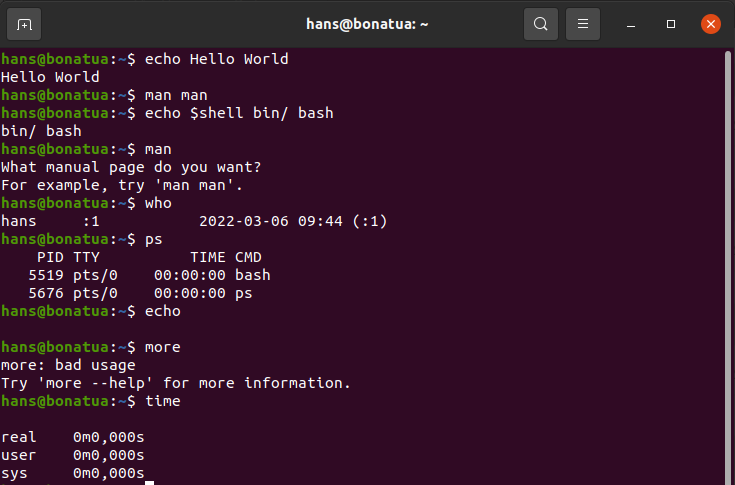
\includegraphics[width=1\textwidth]{Figure/tut1a.png}
		\caption{Percobaan 1.1}
		\label{fig:aug-1}
	\end{subfigure}
	\qquad %add desired spacing between images, e. g. ~, \quad, \qquad, \hfill etc. 
	%(or a blank line to force the subfigure onto a new line)
	\begin{subfigure}[b]{0.4\textwidth}
		\centering
		\def\svgwidth{\columnwidth}
		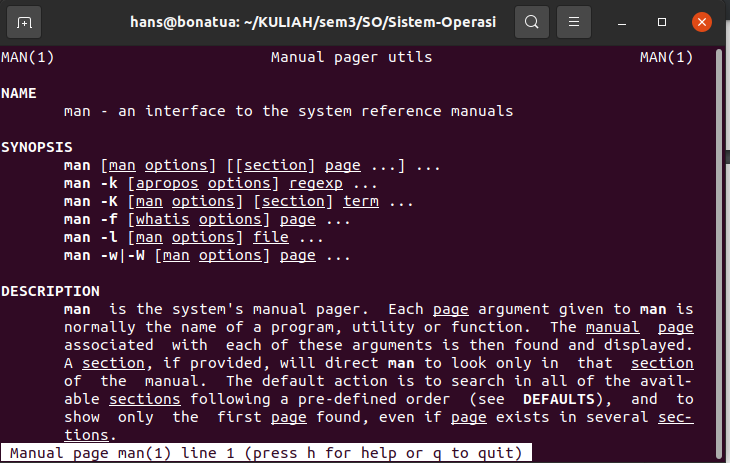
\includegraphics[width=1\textwidth]{Figure/tut1.1.png}
		\caption{Percobaan 1.2}
		\label{fig:aug-2}
	\end{subfigure}
	
\end{figure}

\begin{figure}[h]
    \centering
    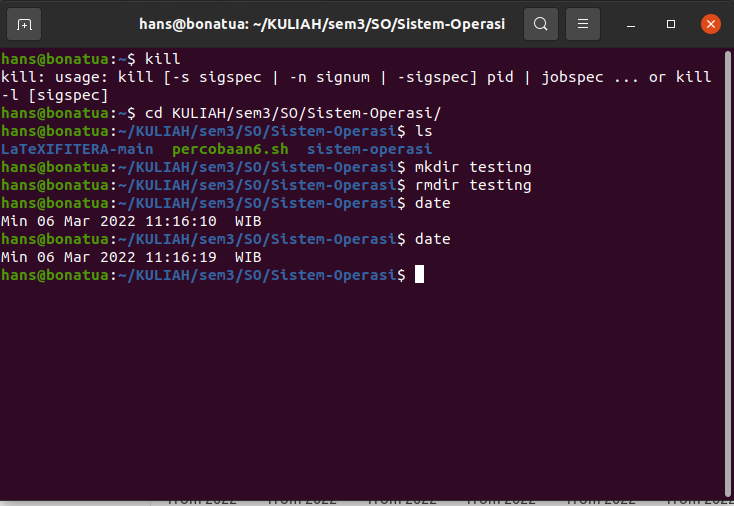
\includegraphics[width=0.4\textwidth]{Figure/tut1b.png}
    \caption{Percobaan 1.3}
\end{figure}


\subsection{Tut 1.4}
pada percobaan yang ada pada gambar kedua ini mencakup pada bagian dari tut1 yang meliputi poin 4, walaupun beberapa poin sudah dikerjakan pada bagian lain,dan selanjutnya mencoba berbagai bentuk sintax yang dapat digunakan oleh pemakai linux dalam mengoperasikan linux khususnya terminal berikut sintax-sintaxnya yang pertama ada kill yang 
berfungsi untuk menghentikan berbagai program yang instan dalam prosesnya, selanjutnya fungsi ada sintax cd yang berfungsi untuk berpindah antar directory, ada sintax ls yang berguna untuk menampilkan isi directory, selanjutnya ada mkdir yang berguna untuk membuat suatu directory, rmdir yang berguna untuk menghapus directory date, yang berguna untuk menampilkan hari dan tanggal berlangsung, selain fungsi diatas dan pada gambar sebelumnya terdapat sintax layout yang berguna untuk kembali kelayout, history untuk menampilkan riwayat pekerjaan, pwd berfungsi untuk mencari posisi directory dan beberapa sintax lagi yang belum dicoba ditut 1namun akan dicoba pada tut selanjutnya
     \begin{figure}[h]
		\centering
		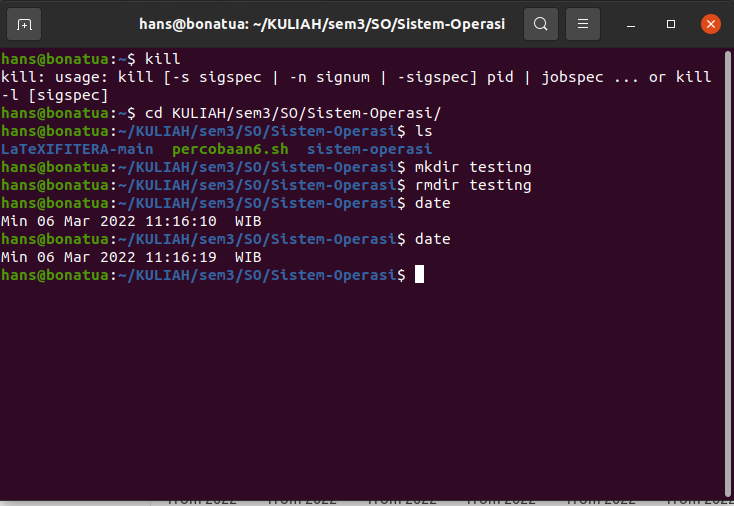
\includegraphics[width=0.6\textwidth]{Figure/tut1b.png}
		\caption{Percobaan Tut 1.4}
	\end{figure}

\section{Laporan Tut 2}
Pada percobaan ini berisi pemakaian perintah sed untuk berfungsi menghapus karakter pertama dan karakter terakhir, awalnya buat terlebih dahulu suatu file bertipe data txt yang diisi dengan kalimat 
dan selanjutnya untuk menampilkan gunakan perintah grep untuk menemukan berapa banyak baris file yang berisi file yang dibuat diawal dengan tujuan untuk menemukan 
kata yang diberikan. Nama film dan kata disediakan sebagai input. dengan ketentuan program yang dipakai untuk menjalankan fungsi tersebut.
    \begin{figure}[h]
        \centering
        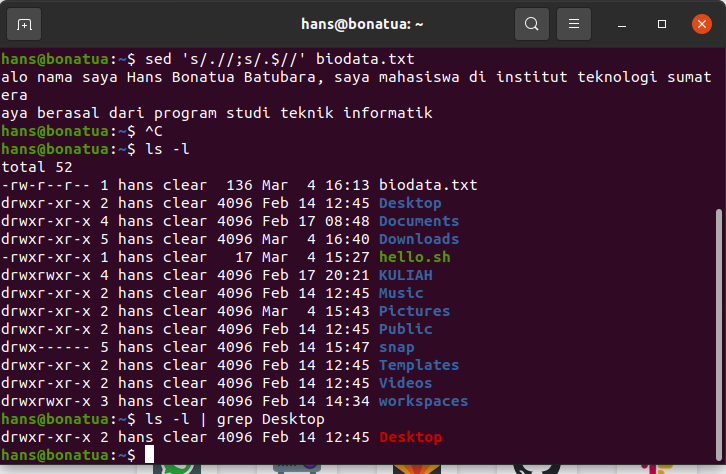
\includegraphics[width=0.6\textwidth]{Figure/tut2.png}
        \caption{Percobaan Tut 2}
    \end{figure}
\newpage
\section{Laporan Tut 3}
pada percobaan tut 3 akan dirancang untuk merujuk ke buku teks tentang skrip shell yang disediakan dibagian file sebelumnya sebelum mencoba
tutorial ini dengan langkah berikut.
\begin{itemize}
    \item Tulis skrip shell untuk menampilkan “HELLO WORLD” di terminal:
    \item Ketik echo HELLO WORLD pada terminal
    \item Simpan file dengan ekstensi .sh ( katakan test.sh)
    \item Tutup editornya
    \item Di terminal, ketik sh test.sh dalam program diatur dengan file lain bernama hello
    \item Output yang diharapkan pada prompt: HELLO WORLD
\end{itemize}
\begin{figure}[h]
    \centering
    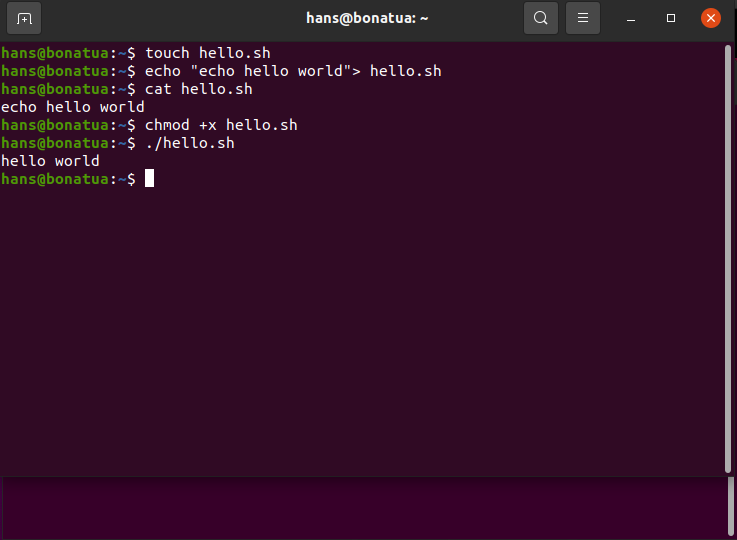
\includegraphics[width=0.6\textwidth]{Figure/tut3.png}
    \caption{Percobaan Tut 3}
\end{figure}

\section{Laporan Pembahasan Tugas - 6}
    \begin{lstlisting}[language=Bash, caption=Program Assignment 6,label={labelkode}]
    ls | tr a-z A-Z
    \end{lstlisting}
    Pada percobaan soal keenan diminta skrip shell yang menerima satu atau lebih nama file sebagai argumen dan mengonversi semuanya menjadi huruf besar, 
    yang ada di direktori saat ini dalam implementasinya kita memakai file hello.txt sebagai media percobaan dengan sinatx diyang ada diterminal.

\section{Laporan Pembahasan Tugas - 8}
    \begin{lstlisting}[language=Bash, caption=Program Assignment 8,label={labelkode}]
    !/bin/sh
    echo "masukkan Nama file"
    read name
    echo "masukkan kata yang akan dihapus"
    read kata
    echo " "
    grep -v $kata $name
    \end{lstlisting}
    Pada percobaan yang ada shell akan  menerima nama file, baris awal dan akhir
    angka sebagai argumen dan menampilkan semua baris berada di antara baris yang diberikan
    angka.

\section{Laporan Pembahasan Tugas - 9}
    \begin{lstlisting}[language=Bash, caption=Program Assignment 9,label={labelkode}]
    #!/bin/sh
    echo "Masukkan nama file "
    read name
    echo "Masukkan awal baris yang ingin dikeluarkan"
    read awal
    echo "Masukkan akhir baris yang ingin dimasukan"
    read akhir
    echo " "
    sed -n $awal,$akhir\p $name | cat > Baris 
    cat Baris
    \end{lstlisting}
    Pada percobaan diawali shell yang menerima nama file, baris awal dan akhir
angka sebagai argumen dan menampilkan semua baris di antara baris yang diberikan
angka. program yang berdasarkan sintax akan bekerja untuk menampilkan semua baris di antara baris.

\section{Kesimpulan}
Dari Hands On pertama ini yang saya dapatkan ialah Linux khususnya ubuntu merupakan salah satu bentuk dari sistem operasi yang memiliki 
kelebihan yakni open source sehingga pemakai linux khususnya ubuntu dapat menambahkan fitur yang dikehendaki seperti percobaan 6 sampai denfgan program 9 dengan linux yang yang dapat dipakai dengan mengabungkan beberapa sintax kita dapat bebas juga mengakses berbagai hal yang ada didalam linux (ubuntu). 
Sintax yang dapat diterapkan menjadi keuntungan tersendiri bagai pemakai dan ringan (minim) tempat penyimpanan data yang ringan

\section{Link Google Drive/ GitHub}
Link GitHub : \href{https://github.com/Hans299}{DISINI}
\bibliographystyle{IEEEtran}
\end{document}